%!TEX root = ../main.tex

In Section~\ref{sec:algorithm}, to deal with the non-register-representable RECL constraints, we unfold all the non-register-representable occurrences of counting operators. Nevertheless, 
the naive unfolding incurs an exponential blow-up over the formula sizes, especially when the counting bounds are large. 
Recall that an occurrence of counting operators is said to be non-register-representable if it is in the scope of some Kleene star, another counting operator, complement, or language difference. Since Kleene star can be seen as a special case of the counting operators, and language difference $e_1 \setminus e_2$ can be rewritten as $e_1 \cap \overline{e_2}$, without loss of generality, we can assume that a non-register representable occurrence of a counting operator is in the scope of another counting operator or some complement operator. 
In the sequel, to alleviate the formula-size blow-up problem resulted from the naive unfolding, we present various optimizations, for the nesting of counting operators and the nesting of counting operators and a complement operator respectively. 
% two situations that a counting operator is in the scope of another counting operator and in the scope of a complement operator respectively. 

\subsection{Optimizations for the nesting of counting operators}\label{heuristic:nested}

In the sequel, we propose an optimization for the nesting of counting operators. 
The optimization is designed for the special case that the nesting depth of counting operators is one. For a RECL constraint whose nesting depth of counting operators is greater than two, we can apply the optimization for the inner-most nesting of counting operators and decrement the nesting depth, then apply the optimization again to the resulting constraint, and continue this process, until obtaining a register-representable RECL constraint.  

The main idea of the optimization is illustrated by the constraint $x \in (a^{\{1,1000\}})^{\{1,2\}}$. If we apply the naive unfolding in Section~\ref{sec:algorithm}, we will unfold  $a^{\{1,1000\}}$ and obtain the constraint $x \in (a(\varepsilon + a + aa + \cdots + \underbrace{a\cdots a}_{999}))^{\{1,2\}}$. It is easy to observe that a smarter way is to unfold  $^{\{1,2\}}$, instead of $^{\{1, 1000\}}$. If we do this, then we get a constraint $x \in (a^{\{1,1000\}})(\varepsilon + a^{\{1,1000\}})$, whose size is much smaller, compared to $x \in (a(\varepsilon + a + aa + \cdots + \underbrace{a\cdots a}_{999}))^{\{1,2\}}$. (Recall that we assume a binary encoding of the integer constants in counting operators.)

Let us describe the optimization more precisely. 
\begin{itemize}
\item For a regular expression $e = (e_1)^{\{m,n\}}$ where $e_1$ is a register-representable regular expression, we can unfold the counting operators in the following ways to obtain a register-representable RECL constraint: (i) unfold the counting operators in $e_1$, (ii) unfold the counting operator $^{\{m,n\}}$. 
%
Let $\ufld_1(e)$ and $\ufld_2(e)$ denote the resulting regular expressions. 

\item We estimate the sizes of the two CEFAs $\aut_{\ufld_1(e)}, \aut_{\ufld_2(e)}$ constructed from $\ufld_1(e), \ufld_2(e)$ respectively as pairs $(\snum_1(e), \rnum_1(e))$ and $(\snum_2(e), \rnum_2(e))$, where $\snum_1(e)$ and $\rnum_1(e)$ are the estimates of the number of states and registers in $\aut_{\ufld_1(e)}$, similarly for $\snum_2(e)$ and $\rnum_2(e)$. 
%
\item From the construction in Section~\ref{sec:algorithm}, 
two NFAs $\cU_{\aut_{\ufld_\hdh{1}(e)}}, \cU_{\aut_{\ufld_2(e)}}$ are constructed from $\aut_{\ufld_1(e)}$ and $\aut_{\ufld_2(e)}$ by dropping the accepting conditions and ignoring the characters. As a result, the alphabets of $\cU_{\aut_{\ufld_\hdh{1}(e)}}, \cU_{\aut_{\ufld_2(e)}}$ are the set of integer vectors occurring in the transitions of $\aut_{\ufld_1(e)}, \aut_{\ufld_2(e)}$ respectively. \hdh{Note that there is only one register in $\aut_{\ufld_1(e)}$. Because each occurrence of the counting operators in $\ufld_2(e)$ originates from the register-representable $e_1$, thus not in the scope of any Kleene star, counting, complement, or language difference, it follows that 
in $\aut_{\ufld_2(e)}$, the registers corresponding to these counting operators are updated independently, that is, the integer vectors of  $\aut_{\ufld_2(e)}$ are of the form $(\underbrace{0, \cdots, 0}_{i-1}, 1, \underbrace{0, \cdots, 0}_{\rnum_1(e)-i-1})$, where $i \in [\rnum_2(e)]$.} Consequently, the size of the alphabet of $\cU_{\aut_{\ufld_1(e)}}$ is bounded by $\rnum_1(e)$. Similarly for $\cU_{\aut_{\ufld_\hdh{2}(e)}}$. 
Finally, we estimate the sizes (number of transitions) of the NFAs $\cU_{\aut_{\ufld_1(e)}}, \cU_{\aut_{\ufld_2(e)}}$ as $sz_1 = (\snum_1(e))^2 \cdot \rnum_1(e)$ and $sz_2 = (\snum_2(e))^2 \cdot \rnum_2(e)$ respectively. \zhilin{to be checked}
%
\item If $sz_1 \le sz_2$, then we choose to unfold the counting operators in $e_1$. Otherwise, we choose to unfold the counting operator $^{\{m,n\}}$. 
\end{itemize}

%In the sequel, we show how we estimate the sizes of CEFAs constructed from register-representable regular expressions. 

It remains to show how to compute the pairs $(\snum_1(e), \rnum_1(e))$ and $(\snum_2(e), \rnum_2(e))$ from $e=(e_1)^{\{m,n\}}$. Let $e=(e_1)^{\{m,n\}}$ be a regular expression where $e_1$ is a register-representable regular expression. Then we compute $\snum'_1(e_1)$ and $(\snum'_2(e_1), \rnum'_2(e_1))$. Finally, let $(\snum_1(e), \rnum_1(e)) = (\snum'_1(e_1), 1)$ and $(\snum_2(e), \rnum_2(e)) = (\snum'_2(e_1), \rnum'_2(e_1))$.
\begin{itemize}
  \item If $e_1 = \emptyset$ or $e_1 = \epsilon$, then $\snum'_1(e_1)  = 0$ and $(\snum'_2(e_1), \rnum'_2(e_1))  = (0, 0)$. 
%
  \item \hdh{If $e_1 = a$, then $\snum'_1(e_1) = 1$ and ($\snum'_2(e_1), \rnum'_2(e_1)) = (n, 0)$.}
 %
  \item If $e_1 = e_2 \concat e_3$, then $\snum'_1(e_1) = \snum'_1(e_2) + \snum'_1(e_3)$ and 
%
  $$
  \begin{array}{l }
 (\snum'_2(e_1), \rnum'_2(e_1)) =  \\
  \ \ \ \ (n(\snum'_2(e_2) + \snum'_2(e_3)), n(\rnum'_2(e_2) + \rnum'_2(e_3))).
 \end{array}
  $$
%
 \item If $e_1 = e_2 + e_3$, then $\snum'_1(e_1) = \snum'_1(e_2) + \snum'_1(e_3)$ and 
%
  $$
  \begin{array}{l }
 (\snum'_2(e_1), \rnum'_2(e_1)) =  \\
  \ \ \ \ (n(\snum'_2(e_2) + \snum'_2(e_3)), n(\rnum'_2(e_2) + \rnum'_2(e_3)+1)).
 \end{array}
  $$
 (Recall that the construction of $\aut_1 \cup \aut_2$ introduces one additional register.)
%
 \item If $e_1 = e_2 \cap e_3$, then $\snum'_1(e_1) = \snum'_1(e_2) \times \snum'_1(e_3)$ and 
%
  $$
  \begin{array}{l }
 (\snum'_2(e_1), \rnum'_2(e_1)) =  \\
  \ \ \ \ (n(\snum'_2(e_2) \times \snum'_2(e_3)), n(\rnum'_2(e_2) + \rnum'_2(e_3))).
 \end{array}
  $$
%
 \item If $e_1 = \overline{e_2}$, then $\snum'_1(e_1) = 2^{\snum'_1(e_2)}$ and 
%
  $
%  \begin{array}{l }
 (\snum'_2(e_1), \rnum'_2(e_1)) =  (n \cdot 2^{\snum'_2(e_2)}, 0).
% \end{array}
  $
 (The exponential blow-up is explained by the fact that the determinization is needed for the complementation.) 
%
%  \item If $\regex = \overline{\regex_1}$, then $s_\regex = 2^{s_{\regex_1}}$ (since the determinization is needed for the complement) and $r_\regex = 0$.
%
 \item If $e_1 = (e_2)^*$, then $\snum'_1(e_1) = \snum'_1(e_2)$ and 
%
  $
%  \begin{array}{l }
 (\snum'_2(e_1), \rnum'_2(e_1)) =  (n \snum'_2(e_2), 0).
% \end{array}
  $
%  \item If $\regex = \regex_1^*$, then $s_{\regex} = s_{\regex_1}$ and $r_{\regex} = 0$.
%  \item $\regex = \regex_1 \backslash \regex_2$ can be transferred to $\regex = \regex_1 \cap \overline{\regex_2}$ and then the size can be computed by the formula of $\cap$ and $\bar{}$.
 \item If $e_1 = (e_2)^{\{m', n'\}}$ or $e_1 = (e_2)^{\{n', \infty\}}$, then $\snum'_1(e_1) = n' \snum'_1(e_2)$ and 
%
  $
%  \begin{array}{l }
 (\snum'_2(e_1), \rnum'_2(e_1)) =  (n \snum'_2(e_2), n).
% \end{array}
  $
%  \item For $\regex = \regex_1^{\{m, n\}}$ or $\regex = \regex_1^{\{n,\infty\}}$, $s_{\regex} = s_{\regex_1}$ and $r_{\regex} = 1$.
\end{itemize}

%The naive approach for nested counting in the paper \cite{Denghang2023} is to unwind all inner counting operators. This approach may generate a large number of states, which is linear to the product of the counting bounds in regex and exponential to the length of the regex. For example, naive unwinding regex $(a^{\{1,1000\}})^{\{1,2\}}$ generate a CEFA containing 1000 states. But if we only unwind the outer counting operator of the regex, not the inner, we obtain a CEFA containing only 2 states. The side effect is that we need two registers to store the information of counting in the inner regex (unwinding of the outer counting operator repeats the inner regex, which also repeats the registers of the inner regex). We present a heuristic to reduce the number of states generated by the unwinding process. The idea is to unwind the counting operator with less bound and fewer side effects firstly. We present the heuristic in the following algorithm.

%%%%%%%%%%%%%%%%%%%%%%%%%%%%%%%%%%
%%%%%%%%%%%%%%%%%%%%%%%%%%%%%%%%%%
\hide{
\medskip
\noindent
\emph{Step 1. (Compute the number of states generated by each counting operator if we unwind it).}

For a regex $\regex$, we can approximate the number of states $size(\regex)$ generated by the following formula: 
\begin{itemize}
  \item If $\regex = \emptyset$ or $\regex = \epsilon$, then $size(\regex) = 0$. 
  \item If $\regex = \regex_1 \cdot \regex_2$ or $\regex = \regex_1 + \regex_2$, then $size(\regex) = size(\regex_1) + size(\regex_2)$.
  \item If $\regex = \regex_1^*$, then $size(\regex) = size(\regex_1)$.
  \item If $\regex = \regex_1 \cap \regex_2$, then $size(\regex) = size(\regex_1)*size(\regex_2)$.
  \item If $\regex = \overline{\regex_1}$, then $size(\regex) = 2^{size(\regex_1)} + 1$.
  \item $\regex = \regex_1 \backslash \regex_2$ can be transferred to $\regex = \regex_1 \cap \overline{\regex_2}$ and then the size can be computed by the formula of $\cap$ and $\bar{}$.
  \item For $\regex = \regex_1^{\{n,m\}}$ or $\regex = \regex_1^{\{m,\infty\}}$, $size(\regex)$ is equal to $m*size(\regex_1)$ if it is unwinded, and $size(\regex_1)$ otherwise.
\end{itemize}

For each counting operator $^{\{n,m\}}$ or $^{\{m,\infty\}}$ with $\regex$ as its subregex, the number of states generated by it is $m*size(\regex)$ if we unwind it.

The formula above is an approximation of the states of CEFA generated by Thompson's construction. Note that the number of states is linear to the bound for the counting operator.

\medskip
\noindent
\emph{Step 2. (Compute the number of registers generated by each counting operator if we unwind it).}

We unwind the counting operator with less bound first. The reason is that the number of states generated by the counting operator is linear to its bound. If we unwind the counting operator with less bound first, the number of states generated by the unwinding process is less. However, the hardness of solving the $\cefadec$ problem is not only relevant to the number of states, but also the number of registers. For a regex $\regex$, we can approximate the number of registers $reg(\regex)$ generated by the following formula:
\begin{itemize}
  \item If $\regex = \emptyset$, $\regex = \epsilon$, $\regex = \regex_1^*$ or $\regex = \overline{\regex_1}$, then $reg(\regex) = 0$.
  \item If $\regex = \regex_1\cdot \regex_2$ or $\regex = \regex_1 \cap \regex_2$, then $reg(\regex) = reg(\regex_1) + reg(\regex_2)$.
  \item If $\regex = \regex_1 + \regex_2$, then $reg(\regex) = reg(\regex_1) + reg(\regex_2) + 1$.
  \item $\regex = \regex_1 \backslash \regex_2$ can be transferred to $\regex = \regex_1 \cap \overline{\regex_2}$ and then the number of registers can be computed by the formula of $\cap$ and $\bar{}$.
  \item For $\regex = \regex_1^{\{n,m\}}$ or $\regex = \regex^{\{m, \infty\}}$, $reg(\regex)$ is equal to $m*reg(\regex_1)$ if it is unwinded, and $1$ otherwise.
\end{itemize}

For each counting operator $^{\{n,m\}}$ or $^{\{m,\infty\}}$ with $\regex$ as its subregex, the number of registers generated by it is $m*reg(\regex)$ if we unwind it.

\medskip
\noindent
\emph{Step 3. (Unwind the counting operator with less bound and fewer registers first).}

In the above two steps, we compute the number of states and registers generated by each counting operator. In some cases, we can unwind the counting operator with less bound and fewer registers directly. But in most cases, there are multiple counting operators where one counting operator has less bound and another counting operator has fewer registers. To consider the number of states and registers at the same time, we can compute the score of each counting operator by the following formula:
\begin{itemize}
  \item $score(\regex) = size(\regex) * (reg(\regex)+1)$.
\end{itemize} 
The reason why we use the product to combine the two factors is that the hardness of the $\cefadec$ problem is highly relevant to the number of variables in the final existential LIA formula, which is linear to the product of the number of states and the number of registers. Using $reg(\regex) + 1$ not $reg(\regex)$ is because the number of registers may be $0$.We unwind the counting operator with the smallest score first. 

\begin{example}
 Consider the regex $(a^{\{1,1000\}})^{\{1,2\}}$. The score of $^{\{1,1000\}}$ is $1000*(0+1) = 1000$ and the score of $^{\{1,2\}}$ is $2*(2+1) = 6$. We unwind the outer counting operator first and obtain a CEFA containing only two states.  
\end{example}
}
%%%%%%%%%%%%%%%%%%%%%%%%%%%%%%%%%%
%%%%%%%%%%%%%%%%%%%%%%%%%%%%%%%%%%



\subsection{Optimizations for the nesting of counting operators and a complement operator}

As mentioned in Section~\ref{sec:algorithm}, if some counting operators are in the scope of a complement operator, it is necessary to unfold these counting operators before the complement operation. The exponential blow-up in the unfolding combined with the blow-up in the complement operation will produce a huge number of states. To alleviate this problem, we propose two approximations of the complement operation, i.e., an under-approximation and an over-approximation, and combine them into a procedure that achieves a nice balance between efficiency and precision. 

Let $e = \overline{e_1}$ be a regular expression, where $e_1$ is a register-representable regular expression. 

\paragraph*{Under-approximation}
%
One way of doing the complement operation is to transform $e_1$ into a regular expression that does not contain counting operators. We compute an under-approximation of $e$ by replacing each occurrence of the counting operators in $e_1$, say $(e_2)^{\{m,n\}}$ or $(e_2^{\{n, \infty\}})$, by $e_2^*$. Let us use $e'_1$ to denote the resulting regular expression. Note that $e'_1$ does not contain counting operators. Moreover, it is easy to observe that $\Lang(e_1) \subseteq \Lang(e'_1)$. As a result, we have $\Lang(\overline{e'_1}) \subseteq \Lang(\overline{e_1})$. That is, $\overline{e'_1}$ is an under-approximation of $\overline{e_1}$. 

%The under-approximation is replacing each counting operator in the subregex of complement with a Kleene star operator. The language of the subregex is a superset of the language of it after under-approximation. In sequential, the complement of the subregex is a subset of the origin. Note that this approach only works for non-nested complement, which means there is no other complement operators in the complement. For nested complement,  we naively handle the inner complement operators as paper \cite{Denghang2023} and then under-approximate the outer complement operator.

\paragraph*{Over-approximation}
For $e = \overline{e_1}$, we utilize the CEFA constructed from $e_1$, say $\aut_{e_1}$, to construct a CEFA $\cB$ of $e$ so that $\Lang(\cB)$ is an over-approximation of $\Lang(e)$. 
Let $\aut_{e_1} = (R, Q, \Sigma, \delta, I, F, \alpha)$. The main idea of the construction is explained as follows: If a string $w$ is not accepted by $\aut_{e_1}$, then either there are no runs of $\aut_{e_1}$ on $w$, or every run of $\aut_{e_1}$ on $w$ stop at a non-final state or enter a final state but do not satisfy the accepting condition $\alpha$. We shall construct a CEFA $\cB$ that accepts when one of these situations occurs. Then $\overline{\Lang(\aut_{e_1})} \subseteq \Lang(\cB)$, that is, $\cB$ is an over-approximation of $e$. 

Without loss of generality, we can assume that there are no transitions out of $F$ in $\aut_{e_1}$. If this is not the case, then a new state $q_f$ can be introduced to transform $\aut_{e_1}$ into a CEFA satisfying this constraint, where $q_f$ is the unique accepting state. 
Then we define $\cB= (R \cup \{r'\}, Q \cup \{q_s\}, \Sigma, \delta', I, Q \cup \{q_s\}, \alpha')$, where
\begin{itemize}
  \item $r'$ is a new register not in $R$, 
  \item $q_s$ is a new state not in $Q$,
  \item $\delta'$ comprises the following transitions, 
  \begin{itemize}
    \item $(q, a, q', (\vec{v}, 0))$ such that $(q, a, q', \vec{v}) \in \delta$ and $q' \not \in F$,
%
    \item $(q, a, q_s,(\vec{0}, 0))$ such that there do \emph{not} exist $a$-labeled transitions out of $q$, that is, for every $q'$ and $\vec{v}$, we have $(q, a, q', \vec{v}) \not\in \delta$,
%
    \item $(q, a, q', (\vec{v}, 1))$ such that $(q, a, q', \vec{v}) \in \delta$ and $q' \in F$,
%
    \item $(q_s, a, q_s, (\vec{0}, 0))$ such that $a \in \Sigma$, 
  \end{itemize}
  \item $\alpha'$ is defined as $r' = 1 \rightarrow \neg \alpha$.
\end{itemize}
Intuitively, $q_s$ is a sink state that deals with the situations where there are no runs, and $r'$ is a register newly introduced so that the different cases of the non-accepting runs of $\aut_{e_1}$ can be captured by a single accepting condition $\alpha'$. 

Note that $\cB$ is a strict over-approximation of $e = \overline{e_1}$ since $\aut_{e_1}$ may be nondeterministic. For instance, if there are two runs of $\aut_{e_1}$ on a string $w$, say one run that ends at a non-final state and another run that ends at a final state and satisfies accepting condition $\alpha$. Then $w \in \Lang(\aut_{e_1})$, thus $w \not \in \Lang(\overline{\aut_{e_1}})$. Nevertheless, according to the construction, $w$ is accepted by $\cB$, witnessed by the run of $\aut_{e_1}$ that ends at a non-final state. 

\hdh{\paragraph*{Combination of under- and over-approximation}
 In our configuration, under-approximation is performed first due to its superior computational efficiency, and we proceed with over-approximation if it yields an unsatisfiable result. When the under-approximation yields an unsatisfiable result and the over-approximation yields a satisfiable result, we employ the decision procedure to obtain an answer, which implies that our approach is sound and complete. To minimize computational overhead, we apply approximation techniques only in cases involving non-register-representable regular expressions with significant counting bounds—specifically, those exceeding 20 in our experimental configuration.
}

%As we mentioned in the above section \ref{heuristic:nested}, the unwinding process of the complement operator is exponential to the counting bounds in the worst case. We present a heuristic to reduce the number of states generated by the unwinding process. The idea is to under-approximate and over-approximate the language of the regex first, so that we can avoid unwinding counting operators in complement. We present the heuristic in the following algorithm.

%%%%%%%%%%%%%%%%%%%%%%%%%%%%%%%%%%%%%
%%%%%%%%%%%%%%%%%%%%%%%%%%%%%%%%%%%%%
\hide{
\medskip
\noindent
\emph{Step 1. (Under-approximate the language of the regex with complement operators).}

The under-approximation is replacing each counting operator in the subregex of complement with a Kleene star operator. The language of the subregex is a superset of the language of it after under-approximation. In sequential, the complement of the subregex is a subset of the origin. Note that this approach only works for non-nested complement, which means there is no other complement operators in the complement. For nested complement,  we naively handle the inner complement operators as paper \cite{Denghang2023} and then under-approximate the outer complement operator.

\medskip
\noindent
\emph{Step 2. (Over-approximate the language of the regex with complement operators).}

The over-approximation is to "complement" the CEFA of the subregex directly, without unwinding the counting operators in the subregex. The over-approximated complementary algorithm for CEFA is as follows:

Given a CEFA $\aut = (R, Q, \Sigma, \delta, I, F, \alpha)$, the over-approximated complement of it is a tuple $(R\cup\{r\}, Q\cup\{s,f\}, \Sigma, \delta', I, (Q\cup\{s,f\})\backslash F, \alpha')$, where :
\begin{itemize}
  \item $r$ is a new regesiter not in $R$.
  \item $s$ and $f$ are two new states not in $Q$.
  \item $\delta'$ is a transitions set containing all transitions in $\delta$ and transitions from each state $q$ in $Q$ to $s$ with label $a$ if there is no transitions from $q$ to any state with label $a$ in $\aut$. To be more detailed, $\delta'$ is the union of four sets:
  \begin{itemize}
    \item $\{(q, a, q',(\vec{v}, 0)) \mid (q, a, q', \vec{v})\in \delta\}$
    \item $\{(q, a, s,(\vec{0}, 0)) \mid \forall q'\in Q,\vec{v}. (q, a, q', \vec{v})\not\in \delta\}$
    \item $\{(q, a, f,(\vec{v}, 1)) \mid \exists q'\in F, (q, a, q', \vec{v})\in \delta\}$
    \item $\{(s, \Sigma, s, (\vec{0}, 0))\}$
  \end{itemize}
  \item $\alpha'$ is $r \not= 1\vee \neg \alpha$
\end{itemize}

$r$ is the register used to check whether the accepted state is also accepted in the original CEFA. $s$ is the self-loop state accepting all strings that are not accepted by the original CEFA. $f$ is the merged accepted state of the original CEFA. If there is a transition $(q, a, q', \vec{v})$ terminating at the accepted state $q'$ in the original CEFA, we add a corresponding transition $(q, a, f, (\vec{v}, 1))$ in the over-approximated complement. From the definition of $\delta'$, we can see that only the transitions goto $f$ increase the value of register $r$. The value of $r$ is $1$ if and only if the accepted state is also accepted in the original CEFA. With the above construction, the meaning of the accepting condition $\alpha'$ is obvious: If the string terminates at the accepting state in the original CEFA, then the accepting condition $\alpha$ is false.

\begin{theorem}
 The language of over-approximated complement of CEFA is a superset of the language of exact complement.
\end{theorem}
\begin{proof}
 Suppose that the original CEFA is $\aut = (R, Q, \Sigma, \delta, I, F, \alpha)$, the over-approximated complement of it is $\overline{\aut}_{over} = (R\cup\{r\}, Q\cup\{s,f\}, \Sigma, \delta', I, (Q\cup\{s,f\})\backslash F, \alpha')$, and the exact complement of it is $\overline{\aut}$. To prove the theorem, we only need to show that if a string is accepted by $\overline{\aut}$, then it is accepted by $\overline{\aut}_{over}$. In other words, we need to show that if a string is not accepted by $\overline{\aut}_{over}$, then it is not accepted by $\overline{\aut}$, which means it is accepted by $\aut$. We prove it by construction.
   
 In the definition of CEFA in section \ref{sec:automaton}, a run $q_0 \xrightarrow[\myvec{\overline{v}_1}]{a_1} q_1 \cdots q_{n-1}\xrightarrow[\myvec{\overline{v}_n}]{a_n} q_n$ is \emph{accepting} by $\overline{\aut}_{over}$ if $q_n \in (Q\cup\{s,f\})\backslash F$ and $\alpha'(\myvec{\overline{v}'}/(R\cup\{r\}))$ is true, where $\myvec{\overline{v}'} = \sum \limits_{j \in [n]} \myvec{\overline{v}_j}$. If a string is not accepted by $\overline{\aut}_{over}$, then each run of the string is not accepting run, which means the run terminates at state $q\in F$ or the accepting condition $\alpha'(\myvec{\overline{v}'}/(R\cup\{r\}))$ is $false$. 
   
 If each run teminates at state $q_f\in F$, suppose that each is of form $q_0\xrightarrow[(\myvec{v_1},\myvec{0})]{a_1}q_1\cdots q_{n-1}\xrightarrow[(\myvec{v_n},\myvec{0})]{a_n}q_f$, where $\myvec{\overline{v}_i}$ is $(\myvec{v_i}, \myvec{0})$ or $(\myvec{v_i}, \myvec{1})$ for $1\leq i\leq n$. Then there is a transition $(q_{n-1}, a_n, q_f, \myvec{v_n})$ in $\delta$ because there is a transition $(q_{n-1}, a_n, q_f, (\myvec{v_n}, \myvec{0}))$ in $\delta'$. So there is a transition $(q_{n-1}, a_n, f, (\myvec{v_n}, \myvec{1}))$ in $\delta'$ based on our construction for $\delta'$. The run $q_0\xrightarrow[(\myvec{v_1},\myvec{0})]{a_1}q_1\cdots q_{n-1}\xrightarrow[(\myvec{v_n},\myvec{1})]{a_n}f$ teminates at the accepting state $f$, contridicting the assumption. 
   
 If each run makes the accepting condition $\alpha'(\myvec{\overline{v}'}/(R\cup\{r\}))$ false, then the negation of the accepting condition $\neg\alpha'(\myvec{\overline{v}'}/(R\cup\{r\}))$ is true. The negation can be rewriten to $(r=1\wedge \alpha)(\myvec{\overline{v}'}/(R\cup\{r\})) = (r=1)(\myvec{\overline{v}'}/(R\cup\{r\}))\wedge \alpha(\myvec{\overline{v}'}/(R\cup\{r\}))$. In our construction, only the transitions terminate at $f$ increase one to the value of $r$, so that the run must end at $f$ to make $r=1$ be true. $\alpha(\myvec{\overline{v}'}/(R\cup\{r\})) = \alpha(\myvec{v'}/R)$ is also need to be true, implying that the run is an accepting run of $\aut$.
\end{proof}
}
%%%%%%%%%%%%%%%%%%%%%%%%%%%%%%%%%%%%%
%%%%%%%%%%%%%%%%%%%%%%%%%%%%%%%%%%%%%

\section{\hdh{Optimizations for model generation}}\label{sec-opt-sol-gen}

\zhilin{Double check}

%\zhilin{TODO: I had troubles to understand the section about optimized model generation. Maybe stating what the technical problem that it is solving is in a more dumb proof way would help., } 
Recall that in Section~\ref{sec:algorithm}, the satisfiability of the original RECL constraint is reduced to the satisfiability of the existential LIA formula
\[
\begin{array}{l}
\bigwedge \limits_{i \in [n]} \left(\psi_{\cC_i}(\fZ_{\costset_{\cC_i}}) \wedge \alpha_i\left[\sum\limits_{\myvec{v} \in \costset_{\cC_i}} \anivarz_{i, \myvec{v}} \myvec{v} \big{/}R_{\cB_i}  \right] \right) \ \wedge \\
\ \ \varphi \left[ \sum\limits_{\myvec{v} \in \costset_{\cC_1}} \anivarz_{1, \myvec{v}} \myvec{v} \big{/}R_{\cB_1}, \cdots, \sum\limits_{\myvec{v} \in \costset_{\cC_n}} \anivarz_{n, \myvec{v}} \myvec{v} \big{/}R_{\cB_n} \right].
\end{array}
\]
Let us use $\theta$ to denote this formula. 
Then we utilize some SMT solver, say Z3, to solve the satisfiability of $\theta$. If Z3 reports ``sat'', then it also returns a model, namely, an assignment $\amodel$ of natural numbers to the free integer variables in $\theta$. Then we utilize $\amodel$ to generate a model $\amodel'$ of the $\cefadec$ problem, i.e., an assignment $\amodel'$ of strings to the string variables so that the conditions in Definition~\ref{def-cefadec} are satisfied. 
In the sequel, let us assume $n=1$ for simplicity.
%and use an example to illustrate
We first describe the naive algorithm of generating $\amodel'$ from $\amodel$. Then we show how we optimize this model generation process. 

%%%%%%%%%%%%%%%%%%%%%%%%%%%%%%%%%%%%%%
%%%%%%%%%%%%%%%%%%%%%%%%%%%%%%%%%%%%%%
\hide{
\begin{example}\label{exmp-model-gen-naive}
The CEFA $\cB_1$ and the corresponding NFA $\cC_1$ are illustrated in Figure~\ref{fig-model-gen-opt}. Moreover, let $\varphi \equiv r_1 = 12$. Since the structure of $\cC_1$ is relatively simple, it is not hard to see that 
$$\psi_{\cC_1}(\anivarz_{1,(1,0)}, \anivarz_{1,(0,1)}) = \anivarz_{1,(1,0)} \ge 2 \wedge \anivarz_{1,(1,0)} \equiv 0 \bmod 2 \wedge  0 \le \anivarz_{1,(0,1)} \le 2.$$ 
Moreover, $\alpha_1[(\anivarz_{1,(1,0)}(1,0) + \anivarz_{1,(0,1)}(0,1)) /(r_1, r_2)] \equiv \anivarz_{1,(1,0)} \ge 10 \wedge \anivarz_{1,(0,1)} = 2$.
Then 
$$
\begin{array}{l c l}
\theta & \equiv & 
\anivarz_{1,(1,0)} \ge 2 \wedge \anivarz_{1,(1,0)} \equiv 0 \bmod 2 \wedge  0 \le \anivarz_{1,(0,1)} \le 2\ \wedge \\
& & \anivarz_{1,(1,0)} \ge 10 \wedge \anivarz_{1,(0,1)} = 2 \wedge 
\anivarz_{1,(1,0)} = 12.
\end{array}
$$
Then $\amodel$ defined by $\amodel(\anivarz_{1,(1,0)}) = 12$ and  $\amodel(\anivarz_{1,(0,1)})= 2$ is a model of $\theta$.

To generate a model $\amodel'$ for $\cefadec$ problem, it is necessary to generate a string $w$ such that $(w, (12, 2))$ is accepted by $\cB_1$. 

\begin{figure}[htbp]
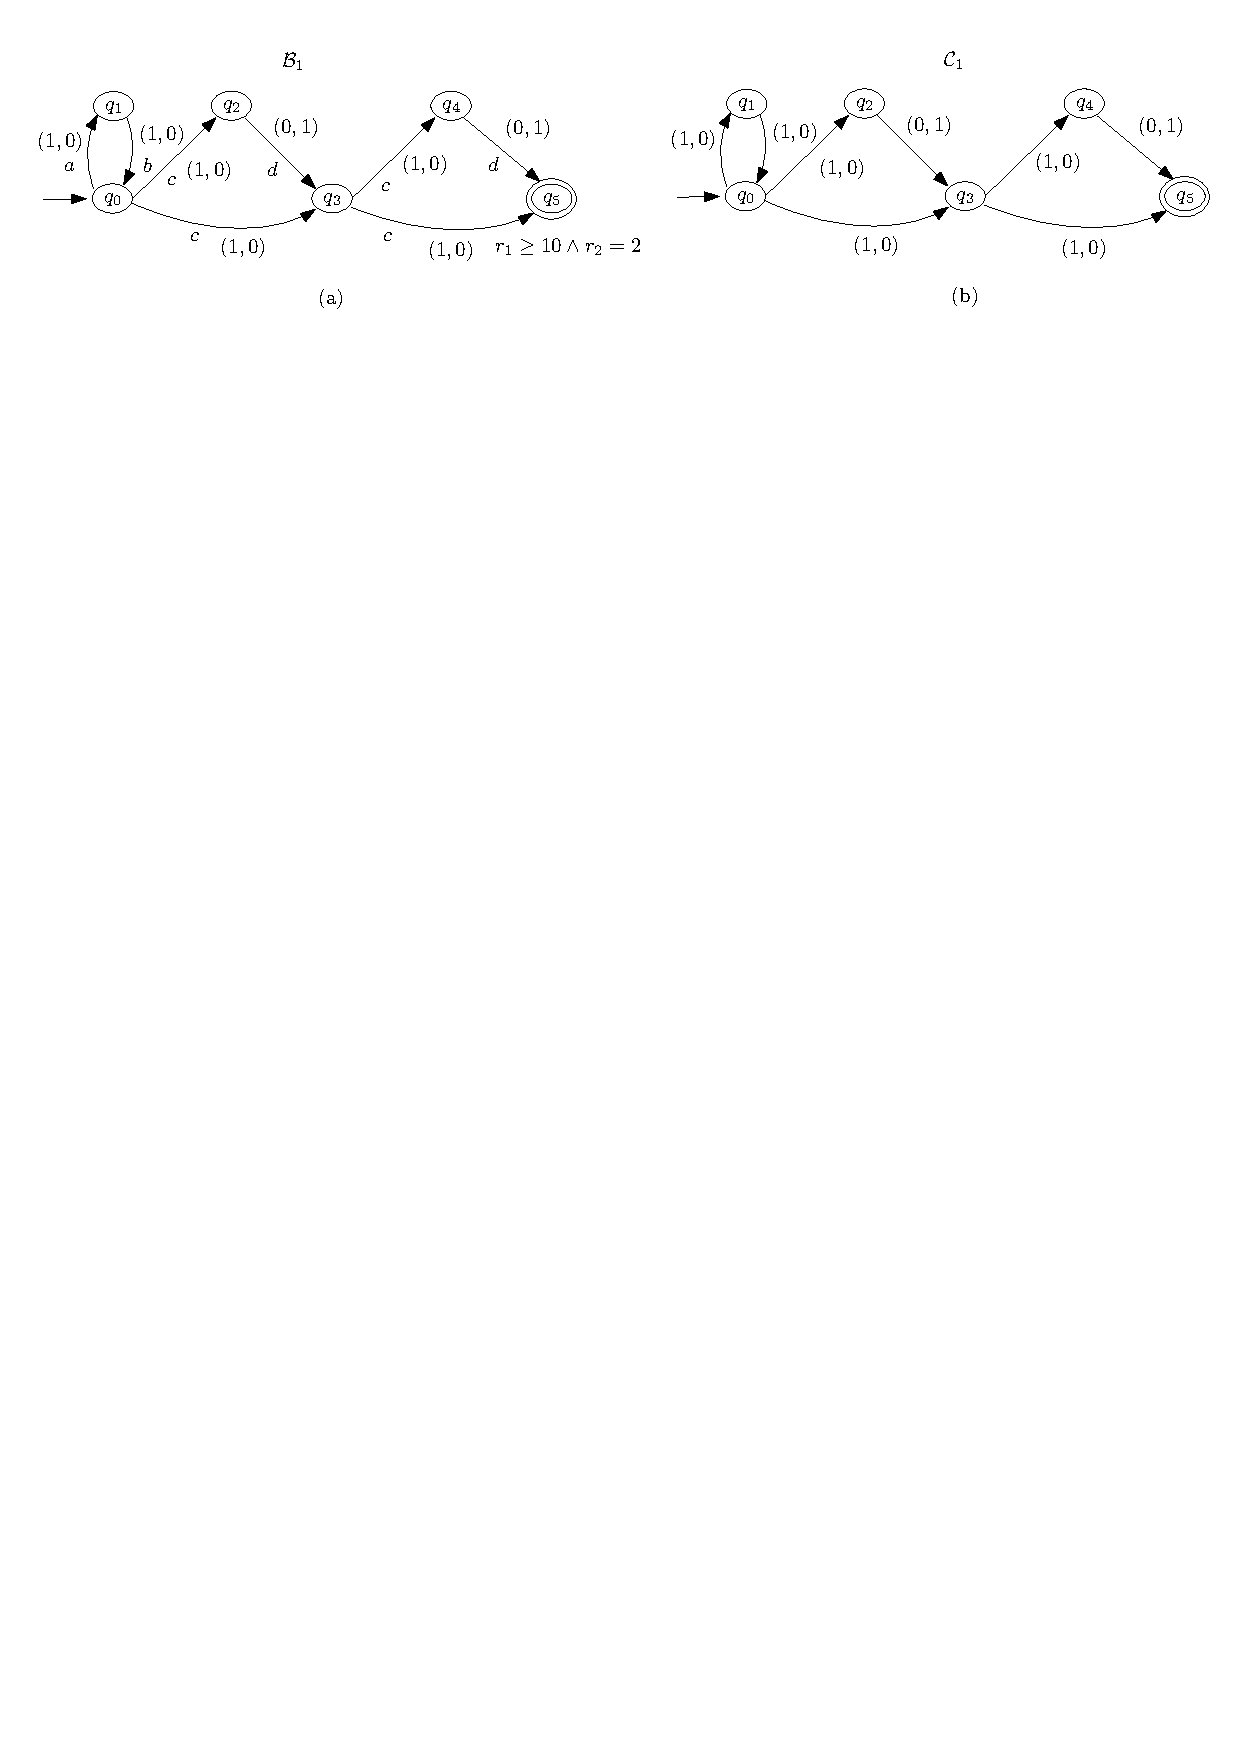
\includegraphics[scale = 0.65]{2024-5-13/sections/model-gen-exmp.pdf}
\caption{The CEFA $\cB_1$ and the NFA $\cC_1$}
\label{fig-model-gen-opt}
\end{figure}
\end{example}
}
%%%%%%%%%%%%%%%%%%%%%%%%%%%%%%%%%%%%%%
%%%%%%%%%%%%%%%%%%%%%%%%%%%%%%%%%%%%%%

\paragraph*{A naive algorithm for model generation}
%For each $i \in [n]$, 
The free variables $\fZ_{\costset_{\cC_1}}$ in $\theta$ correspond to the number of occurrences of characters in $\costset_{\cC_1}$, i.e. the alphabet of the NFA $\cC_1$. Moreover, in $\cC_1$, the characters are just the integer vectors and the characters in the original CEFAs $\cB_1$ used to construct $\cC_1$ are ignored. 
We then utilize $\amodel$ and the CEFA $\cB_1$ to generate $\amodel'$. Essentially, we are solving the reachability problems in a finite transition system where 
\begin{itemize}
\item the nodes are of the form $(q, (\nvec_{1, \myvec{v}})_{v \in \costset_{\cC_1}})$,
%
\item the transitions are of the form 
$$((q, (\nvec_{1, \myvec{v}})_{\myvec{v} \in \costset_{\cC_1}}), (q, a, q', \myvec{u}), (q', (\nvec'_{1, \myvec{v}})_{\myvec{v} \in \costset_{\cC_1}}))$$
such that $(q, a, q', \myvec{u})$ is a transition in $\cB_1$, $\nvec'_{1, \myvec{u}} = \nvec_{1, \myvec{u}}-1$, moreover, $\nvec'_{1, \myvec{v}} = \nvec_{1, \myvec{v}}$ for every $\myvec{v} \neq \myvec{u}$. 
\end{itemize}
Moreover, the initial and final state of the reachability problem are set to be $(q_0, (\amodel(\anivarz_{1, \myvec{v}}))_{\myvec{v} \in \costset_{\cC_1}})$ and $(q_f, (0,\cdots, 0))$ for some initial state $q_0$ and final state $q_f$. 
Note that the transition system contains exponentially many nodes. As a result, the searching process takes \emph{doubly exponential time} in the worst case, since there are at most doubly exponentially many paths. To alleviate the path-explosion problem, in the sequel, we propose two techniques to reduce the number of transitions of the transition system. 

\hide{
we record the remaining occurrences of vectors $\myvec{v}$ in the transitions of the CEFAs $\cB_1$ as a number $\nvec_{1, \myvec{v}}$ and
each time when a transition $(q, a, q', \myvec{v})$ in $\cB_1$ is traversed, $\nvec_{1, \myvec{v}}$ is decremented. Initially $\nvec_{1, \myvec{v}}$ is set to $\amodel(\anivarz_{1, \myvec{v}})$. The searching process terminates when $\nvec_{1, \myvec{v}}$ becomes $0$ for every $\myvec{v}$. We record the characters in the traversed transitions and obtain a string for the string variable $x_i$ when the searching process terminates. As a result, we obtain a model of $\cefadec$ in the end. Note that the searching process can be seen as solving the reachability problem in a finite-state transition system where the nodes are of the form $(q, (\nvec_{1, \myvec{v}}))$ and the transitions are 
is nondeterministic since there may be multiple transitions 
}
%\hdh{In the worst case, we need search O($\prod_{i=0}^{n} \amodel(\anivarz_{i, \myvec{v}})$) times to find an accepted word.}

%%%%%%%%%%%%%%%%%%%%%%%%%%%%%%%%%%%%%%%%%
%%%%%%%%%%%%%%%%%%%%%%%%%%%%%%%%%%%%%%%%%
\hide{
\begin{example}\label{exmp-model-gen-naive-2}
There are two distinct vectors $(1,0)$ and $(0,1)$ in $\cC_1$. 
The searching process starts from the state $(q_0, (12, 2))$, where $\nvec_{1, (1,0)} = 12$ and $\nvec_{1, (0,1)} = 2$. There are three transitions out of $q_0$, $(q_0, a, (1,0), q_1)$, $(q_0, b, (1,0), q_2)$, $(q_0, c, (1,0), q_3)$. 
\begin{itemize}
\item If the searching process chooses the transition $(q_0, a, (1,0), q_1)$, then the state $(q_1, (11,2))$ is reached and a letter $a$ is added to the end of the string (to be generated). 
%
\item If the searching process chooses the transition $(q_0, c, (1,0), q_2)$, then the state $(q_2, (11,2))$ is reached and a letter $c$ is added to the end of the string  (to be generated).
%
\item If the searching process chooses the transition $(q_0, c, (1,0), q_3)$, then the state $(q_3, (11,2))$ is reached and a letter $c$ is added to the end of the string  (to be generated).
\end{itemize}
The searching process continues from the state $q_1$, $q_2$, and $q_3$ respectively. If a state $(q_5, (n_1,n_2))$ such that $n_1 > 0$ or $n_2 > 0$ is reached, then some wrong choices have been made before and the searching process should be backtracked. If a state $(q_5, (0,0))$ is reached, then a desired model is found.  
\end{example}
Note that since we do not have the information about the number of occurrences of the transitions out of $q_0$, starting from the state $(q_0, (12, 2))$, we have to search all the three transitions out of $q_0$. 
}
%%%%%%%%%%%%%%%%%%%%%%%%%%%%%%%%%%%%%%%%%
%%%%%%%%%%%%%%%%%%%%%%%%%%%%%%%%%%%%%%%%%


At first, we refine the states of the transition system by recording the number of transitions, instead of just the number of occurrences of the integer vectors. 

\paragraph*{Refining the states of the transition system by recording the number of transitions}
We shall construct the formula $\theta'$ so that a model of $\theta'$ includes the information about the number of occurrences of the transitions of $\cB_1$.
\[
\begin{array}{l c l}
\theta'  & \equiv &  \psi_{\cB_1}(\fZ_{\cB_1}) \wedge \bigwedge \limits_{\myvec{v} \in \costset_{\cC_1}} \anivarz_{1, \myvec{v}} = \amodel(\anivarz_{1, \myvec{v}}) \ \wedge \\
& & \ \ \bigwedge \limits_{\myvec{v} \in \costset_{\cC_1}} \anivarz_{1, \myvec{v}} = \sum \limits_{(q, a, q') \mbox{ s.t. } (q, a, q', \myvec{v}) \mbox{ is a transition in } \cB_1} \anivarz_{1, (q, a, q', \myvec{v})},
\end{array}
\]
where $\fZ_{\cB_1} = \{\anivarz_{1, (q, a, q', \myvec{v})} \mid (q, a, q', \myvec{v}) \mbox{ is a transition in } \cB_1\}$ is the set of variables $\anivarz_{1, (q, a, q', \myvec{v})}$ denoting the number of occurrences of $(q, a, q', \myvec{v})$. 
Note that compared to $\theta$, $\theta'$ uses the LIA formula $\psi_{\cB_1}$, which is constructed from $\cB_1$ by ignoring its accepting condition and taking it as an NFA where the alphabet is seen as the set of transitions.  Moreover, $\theta'$ relates the values of the variables $\anivarz_{1, \myvec{v}}$ and $\anivarz_{1, (q, a, q', \myvec{v})}$, as well as restricts that the values of $\anivarz_{1, \myvec{v}}$ should be $\amodel(\anivarz_{1, \myvec{v}})$. We then submit $\theta'$ to some SMT solver, which returns a model for $\theta'$, in particular, the values of the variables $\anivarz_{1, (q, a, q', \myvec{v})}$. Equipped with the model, we refine the transition system by considering the nodes $(q, (\nvec_{1, (q, a, q', \myvec{v})})_{(q, a, q', \myvec{v})\mbox{ is a transition in } \cB_1})$, where $\nvec_{1, (q, a, q', \myvec{v})}$ denotes the number of remaining occurrences of $(q, a, q', \myvec{v})$. Note that this refinement can reduce the number of transitions. For instance, if $\nvec_{1, (q, a, q', \myvec{v})} = 0$ for some $(q, a, q', \myvec{v})$, then we can avoid searching the transition $(q, a, q', \myvec{v})$ out of $q$. On the other hand, if in the original transition system where $\nvec_{1, \myvec{v}}$ is used, then it may be the case that we have $\nvec_{1, \myvec{v}} > 0$ (since there may be multiple transitions associated with $\myvec{v}$) and the transition $(q, a, q', \myvec{v})$ should still be searched. 


%%%%%%%%%%%%%%%%%%%%%%%%%%%%%%%%%%%%%%%%
%%%%%%%%%%%%%%%%%%%%%%%%%%%%%%%%%%%%%%%%
\hide{
\begin{example}\label{exmp-model-gen-naive-3}
Let us continue Example~\ref{exmp-model-gen-naive-2}.
$$
\begin{array}{l c l}
\theta' & \equiv & 
\anivarz_{1,(1,0)} \ge 2 \wedge \anivarz_{1,(1,0)} \equiv 0 \bmod 2 \wedge  0 \le \anivarz_{1,(0,1)} \le 2\ \wedge \\
& & \anivarz_{1,(1,0)} \ge 10 \wedge \anivarz_{1,(0,1)} = 2 \wedge 
\anivarz_{1,(1,0)} = 12\ \wedge \\
& & \anivarz_{1,(1,0)} = \anivarz_{1, (q_0, a, q_1, (1,0))} + \anivarz_{1, (q_1, b, q_0, (1,0))} + \anivarz_{1, (q_0, c, q_2, (1,0))} +\\
& & \ \ \ \ \ \ \ \ \ \ \  \anivarz_{1, (q_0, c, q_3, (1,0))} + \anivarz_{1, (q_3, c, q_4, (1,0))} + \anivarz_{1, (q_3, c, q_5, (1,0))}\ \wedge\\
& & \anivarz_{1,(0,1)} = \anivarz_{1, (q_2, d, q_3, (0,1))} + \anivarz_{1, (q_4, d, q_5, (0,1))}.
\end{array}
$$
A model of 
\end{example}
}
%%%%%%%%%%%%%%%%%%%%%%%%%%%%%%%%%%%%%%%%
%%%%%%%%%%%%%%%%%%%%%%%%%%%%%%%%%%%%%%%%


\hide{
It turns out that this model generation process is inefficient, mainly due to the fact that the information about the occurrences of vectors $\myvec{v}$ in $\cB_i$ in the searching process is too coarse. In the sequel, we would like to refine this process by using the number of occurrences of transitions, instead of just the occurrences of integer vectors, to guide the search process. 
Specifically, for each $i \in [n]$ and each transition $(q, a, q', \myvec{v})$ in $\cB_i$, we introduce an integer variable $\anivarz_{i, (q, a, q', \myvec{v})}$ to denote the number of occurrences of the transition, and solve the satisfiability of the following formula,  
\[
\begin{array}{l}
\bigwedge \limits_{i \in [n]} \left(\psi_{\cC_i}(\fZ_{\costset_{\cC_i}}) \wedge \alpha_i\left[\sum\limits_{\myvec{v} \in \costset_{\cC_i}} \anivarz_{i, \myvec{v}} \myvec{v} \big{/}R_{\cB_i}  \right] \right) \ \wedge \\
\ \ \varphi \left[ \sum\limits_{\myvec{v} \in \costset_{\cC_1}} \anivarz_{1, \myvec{v}} \myvec{v} \big{/}R_{\cB_1}, \cdots, \sum\limits_{\myvec{v} \in \costset_{\cC_n}} \anivarz_{n, \myvec{v}} \myvec{v} \big{/}R_{\cB_n} \right]\ \wedge \\
\ \ \bigwedge \limits_{i \in [n]} \bigwedge \limits_{\myvec{v} \in \costset_{\cC_i}} \anivarz_{i, \myvec{v}} = \sum \limits_{(q, a, q', \myvec{v}) \mbox{ occurs in } \cB_i} \anivarz_{i, (q, a, q', \myvec{v})}.
\end{array}
\]
If an SMT solver reports that the aforementioned formula is satisfiable, then the solver can also return a model, which assigns to each variable $\anivarz_{i, (q, a, q', \myvec{v})}$ a natural number. 
%For each $i \in [n]$ and each transition $(q, a, q', \myvec{v})$ in $\cB_i$, let us use $nt_{i, (q, a, q', \myvec{v})}$ to denote the value of $\anivarz_{i, (q, a, q', \myvec{v})}$ in the model.
Then we utilize these values to generate a model (an assignment of strings to string variables) of $\varphi$. 
Let $i \in [n]$. We use a function $\lambda_i$ to record the number of occurrences of the transitions in $\cB_i$. During the search process for $\cB_i$, each time when a transition $(q, a, q', \myvec{v})$ is traversed, $\lambda_i$ is updated by decrementing $\lambda_i((q, a, q', \myvec{v}))$, moreover, $a$ is also recorded. Initially, for each $i \in [n]$ and each transition $(q, a, q', \myvec{v})$ in $\cB_i$, $\lambda_i((q, a, q', \myvec{v}))$ is set to be the value of $\anivarz_{i, (q, a, q', \myvec{v})}$ in the model. When a final state of $\cB_i$ is reached and $\lambda_i((q, a, q', \myvec{v}))$ becomes zero for each transition $(q, a, q', \myvec{v})$ in $\cB_i$, then a desired string is generated for the string variable $x_i$. 
}


Moreover, we propose a method to reduce the number of transitions in the transition system further. 

\paragraph*{Pruning the transitions in the transition system}
%Let $i \in [n]$. 
Let the current state of the transition system be $(p, (\nvec_{1, (q, a, q', \myvec{v})})_{(q, a, q', \myvec{v})\mbox{ is a transition in } \cB_1})$. 
Let us compute the set of transitions of $\cB_1$ that are reachable from the state $p$. Let $\cT_p$ denote this set. If $\{(q, a, q', \myvec{v}) \mid \nvec_{1, ((q, a, q', \myvec{v}))} > 0\} \not \subseteq \cT_p$, then we know that it is impossible to continue the search process so that a string accepted by $\cB_1$ will be found and meanwhile the constraint on the number of transitions enforced by $\nvec_{1, (q, a, q', \myvec{v})}$ is satisfied. Therefore, in this case, we can remove all the transitions out of $(p, (\nvec_{1, (q, a, q', \myvec{v})})_{(q, a, q', \myvec{v})\mbox{ is a transition in } \cB_1})$ and the search halts in this state and is backtracked. 

%\zhilin{stopped here}

%%%%%%%%%%%%%%%%%%%%%%%%%%%%
%%%%%%%%%%%%%%%%%%%%%%%%%%%%
\hide{
In the section \ref{sec:algorithm}, we present an algorithm to solve the $\cefadec$ problem. The algorithm computes existential LIA formulas and then uses an SMT solver to solve them. However, this procedure only answers the question of whether the language of the regex is empty or not. If the language is not empty, we need to find a word in the language in practice. In our previous paper \cite{Denghang2023}, we do not explicitly present the algorithm to find a word in the language because of space limitation. We used a naive approach, which randomly searched the CEFAs by the depth-first search based on the register values obtained from solving the existential LIA formula. However, this approach is not efficient when the regexes are non-register-representable. Suppose that there are $n$ registers whose values are $r_1,\cdots, r_n$ respectively in the CEFA. We may visit each transition $O(r_1*r_2\cdots *r_n)$ times during the search. To relieve this problem, we present a heuristic to find a word in the language as follows.

\medskip
\noindent
\emph{Step 1. (Compute the transitions times visited by the accepted string of CEFAs).}

For each CEFA $\aut = (R, Q, \Sigma, \delta, I, F, \alpha)$, we already know the values of its registers after solving the existential LIA formula. The values can be seen as a constant vector of length $|R|$. We use $\myvec{R}$ to denote the vector and use $\eta((q, a, q', \myvec{v}))$ to denote the parikh image of $\aut$. Then the transition times visited by the accepted string are obtained from the following formula:
$$ \sum \limits_{(q, a, q', \myvec{v})\in \delta} \eta((q, a, q', \myvec{v}))\myvec{v} = \myvec{R}$$

\medskip
\noindent
\emph{Step 2. (Prune the search tree early by the transition times during the search process).}

After computing the transition times visited by the accepted string, we prune the search tree of the CEFA based on the transition times. The idea is that we only visit the state which is able to reach all transitions need to be visited. Other states are deleted from the CEFA so that we can reduce the search space.
Note that the transition times are updated during the search process, so the search space is reduced dynamically. The pseudo-code is presented in Algorithm~\ref{alg:findword}.

\begin{algorithm}[H]
  \caption{Find a word in the language of a CEFA}\label{alg:findword}
  \begin{algorithmic}[1]
  \Procedure{findmodel}{$\aut,tmap$}
  % \State \Comment{$tmap$ maps transition to its remaining visited times}
      \State $todo \gets Stack(\aut_{init}, tmap, '''')$
      \State $visited \gets \emptyset$
      % \State \Comment{a stack of state, remaining visited times and word}
      \While{$todo$ is not empty}
        \State $(q, tmap, w) \gets todo.pop()$
        \If{$q\in \aut_{final}$ and $tmap.values = \myvec{0}$}
          \State \Return $w$
        \EndIf
        
        \For{each transition $(q, a, q', \myvec{v})$ where $tmap[(q, a, q', \myvec{v})]>0$}
          \State $tmap'[(q, a, q', \myvec{v})] \gets tmap[(q, a, q', \myvec{v})] - 1$
          \If{$(q', tmap')\not\in visited$ \textbf{and} \textsc{isReachable}($\aut, q', tmap'$)}
            \State $todo.push((q', tmap', w\cdot a))$
            \State $visited.add((q', tmap'))$
          \EndIf
        \EndFor
      \EndWhile
      \State \Return $\emptyset$ 
  \EndProcedure
  \end{algorithmic}
  \end{algorithm}

 The procedure \textsc{findmodel} takes a CEFA $\aut$ and a transitions-times map $tmap$ as input. $tmap$ maps each transition to its remaining visited times. Stack $todo$ contains states need to be visited, their corresponding transitions-times maps and the current word. Set $visited$ is used to store the visited state with the corresponding map. $todo$ is initialized with the initial state of the CEFA, the input map $tmap$ and an empty word (line 2). $visited$ is initialized as an empty set (line 3).
 In the while loop from line 4 to line 16, the state combined with its transitions-times map is searched by the depth-first search algorithm. During the search process, the procedure returns the word if the state is an accepting state and all remaining times of transitions are $0$ (line 7). For each transition $(q, a, q', \myvec{v})$ whose remaining times are greater than $0$, the procedure decreases the remaining times by $1$ (line 10) and checks whether $(q', tmap')$ is not visited and $tmap'$ is reachable from $q'$ (line 11). We say that \textit{$tmap'$ is reachable from $q'$} if each transition $t$ with $tmap'(t)> 0$ is reachable from the state $q'$. The reachability check (Algorithm~\ref{alg:isReachable}) is vital to prune the search space and reduce the search time. If the state $q'$ is not visited and $tmap'$ is reachable from $q'$, then we push $(q', tmap', w\cdot a)$ to $todo$ and add $(q', tmap')$ to $visited$ to continue the search(line 12-13). If the while loop terminates without finding an accepting word, the procedure returns $\emptyset$ (line 17).  
  
  \begin{algorithm}[H]
    \caption{Check whether the map is reachable from the state}\label{alg:isReachable}
    \begin{algorithmic}[1]
      \Procedure{isReachable}{$\aut, q, tmap$}
      \State $todo \gets Stack(q)$
      \State $visited \gets \emptyset$
      \State $qreach \gets \emptyset$
      \While{$todo$ is not empty}
        \State $q \gets todo.pop()$
        \State $visited.add(q)$
        \For{each transition $t=(q,a,q',\myvec{v})$ where $tmap(t)>0$}
          \State $qreach.add(t)$
          \If{$q'\not\in visited$}
            \State $todo.push(q')$
          \EndIf
        \EndFor
      \EndWhile
      \State Select all transitions $t$ where $tmap(t)>0$ to set $T$
      \If{$T\subseteq qreach$}
        \State \Return \textit{true}  
      \Else 
        \State \Return \textit{false}
      \EndIf
      \EndProcedure
    \end{algorithmic}
  \end{algorithm}

 In Algorithm~\ref{alg:isReachable}, all transitions reachable from the state $q'$ are computed and saved to $qreach$. If $qreach$ covers all transitions with positive times in the input map $tmap$, then we say that $tmap$ is reachable from $q'$ and the procedure \textsc{isReachable} returns true, otherwise it returns false.  
}
%%%%%%%%%%%%%%%%%%%%%%%%%%%%
%%%%%%%%%%%%%%%%%%%%%%%%%%%%
